\documentclass[11pt]{article}
\usepackage{amssymb}

\usepackage{fullpage,times,hyperref,hypcap,namedplus}
\usepackage{cite,enumitem,graphicx,amsmath,algorithmicx,algpseudocode}

\hypersetup{colorlinks=true,allcolors=black}

\title{\bf Identifying Phenotypically Similar Clusters Between Single Cell RNA-Seq Samples}
\author{\bf Guilherme de Sena Brandine}
\date{\today}

\begin{document}

\maketitle

\section{Motivation}
With the increasingly large throughput of single cell RNA-Seq technologies, it is possible to understand the transcriptomes heterogeneous populations of cells in tissues in single-cell resolution. These transcriptomes can be used to identify the phenotype of each sampled cell through diverse methods, such as the expression of specific known marker genes or unsupervised clustering methods based on expression similarity. \\
\\
A question that arises with these technologies is how biological systems differ between two samples, for instance: The differences between the phenotypes of a healthy and a diseased tissues or the differences in a tissue on distinct timepoints of development. We would like to identify which phenotypes are present in  both samples and which are specific to a single one. This could be useful not only to better understand the changing compositions of cell types but also to interrogate the difference between the gene expression of cells of the same phenotype when in different environments. \\
\\
We consider two groups of cells in two different samples to be phenotypically equivalent by weighing in on two factors:

\begin{enumerate}
\item They have similar features.
\item Their relationship to other clusters in the same dataset is similar. 
\end{enumerate}

\section{Measuring Comparability of Complete Euclidean Graphs}
When comparing two sets of clusters from distinct datasets, the first question that arises is whether the two sets are comparable, that is, if the two graphs were overlapped in the best possible way, how similar would the resulting edges be? \emph{(And as soon as I know a way to answer this yes or no question I will write more here)}

\section{Matching Nodes on Comparable Graphs}
We henceforth work on the assumption that we rejected the hypothesis that the graphs are not comparable and we can find a suitable mapping of the nodes. We formalize the problem as such:\\
\\
We take as an input two datasets composing the centroids of the clusters in the two datasets: $X_i = \{x_1, \dots, x_{k_i} \in \mathbb{R}^{n_i}\}$, $i \in \{1,2\}$ where $k_i$ is the number of clusters in dataset $i$ and $n_i$ is the dimension of dataset $i$. Let $N = n_1 + n_2$. A \textbf{matching} between the two datasets is a pair of functions $c_i : X_i \to \{1, \dots, N\}$ that assigns indices (henceforth called ``colors'' for a more visual description) to each cluster in both datasets. Intuitively, we want to assign the same color to clusters that are similar in the two datasets, both in \textbf{content} (values of features) and \textbf{structure} (relationship to other clusters on the same dataset).\\
\\
A \textbf{valid matching} is a matching with the following property: If there is more than one cluster in dataset $i$ with some color $u$, then there exists exactly one cluster in $j \neq i$ with that same color. In practice, this means that two clusters in the same dataset will have the same color if and only if they are subclusters of exactly one cluster in its counterpart dataset. This forbids the ``many-to-many'' relationship between clusters, as well as the same coloring of two clusters in the same dataset with no matching cluster on its counterpart (``many-to-zero'' relationship).

\section{Measuring Valid Matching Quality (Q)}
We propose a formula that measures the quality of a valid matching by weighing in the following quantities:

\begin{itemize}
\item Distance between clusters of equal colors and different datasets (A)
\item Difference between edge values in different datasets that connect clusters of equivalent colors (B)
\item Total distance of clusters with unique colors. (C)
\end{itemize}
Hence, given two datasets $X_1, X_2$, a candidate matching $c_1, c_2$ and a distance metric $|| \cdot ||$, the formula to minimize is given by:
$$
Q(X_1, X_2, c_1, c_2, ||\cdot||) = \sigma_1 A + \sigma_2 B + \sigma_3 C
$$
\\
Where $\sigma_j \in [0,1]$ are the weight factors, that is, $\sigma_1 + \sigma_2 + \sigma_3 = 1$. \\
\\
We call $c_1$ and $c_2$ an \textbf{optimal valid matching} for datasets $X_1$ and $X_2$ if it minimizes $Q$ over all possible valid matchings. 
\\
\\
We will now describe how to calculate the 3 factors(A, B and C) above:

\subsection{The factor A (content similarity)}
$A$ is calculated by iterating over all colors that exist on both datasets simultaneously and calculating their distances. Since the matching is valid, each color will appear only once in at least one of the datasets. We define the matched colors as the intersection of the images of both functions $c_i$, that is: $S = S_1 \cap S_2$, where $S_i = \mbox{Im} (c_i)$. Similarly, we define $c_{i}^{-1}(k) = \{x \in X_i | c_i(x) = k\}$ as the set of all clusters in dataset $X_i$ whose color is $k$. We thus have:

$$
A = \sum_{\substack{k \in S}} \sum_{\substack{x_i \in c_{i}^{-1}(k) \\ x_j \in c_{j}^{-1}(k)}} \frac{||x_i - x_j||^2}{|c_{i}^{-1}(k)| |c_{j}^{-1}(k)|}
$$
\\
Note that in this formula, if the same color appears $m$ times in a dataset, we will calculate average of the $m$ distances from the same color cluster to its equivalent counterpart. This penalizes merging clusters that are very far away into a midpoint cluster that turns the two graphs ``more isomorphic'' just by chance. 

\subsection{The factor B (structure similarity)}
$B$ measures how well the matching encodes the candidate isomorphism of the two datasets. For this, every color present multiple times in a dataset will be \textbf{collapsed} into its centroid. In the previous section, we used the notation $c_{i}^{-1} (k)$ to represent all the clusters in dataset $X_i$ whose color is $k$. Here will slightly abuse the notation and use $c_{i}^{-1} (k)$ as the average of all elements in this set.\\
\\
With that said, Let $S^2 = S\times S$ be the set of all pairs of colors present in both datasets. B is then given by:

$$
B = \sum_{\substack{(k,l) \in S^2 \\ k \neq l}} (||c_{1}^{-1}(k) - c_{1}^{-1} (l)|| - ||c_{2}^{-1}(k) - c_{2}^{-1} (l)||)^2
$$
\\
This means we calculate the difference between the weights of edges whose endpoints have matching colors. $B=0$ if and only if all edges that connect endpoints of the same color are the same in both datasets. 

\subsection{The factor C (unmatched cluster penalty)}
$C$ encodes the penalty from clusters that have an unique unmatched color. Since each unique color has no candidate isomorph on the counterpart dataset, we propose to penalize it by summing its distance to all clusters on its dataset. We define the unique color sets as $T_i = S_i - S$. $C$ is then calculated by:

$$
C = \sum_{\substack{i \in \{1,2\}}} \sum_{\substack{k \in T_i}} \sum_{\substack{x_i \in X_i \\ x_i \neq c_{i}^{-1}(k) }} \frac{ (c_{i}^{-1} (k) - x_i)^2}{|X_i| - 1}
$$
Note that since the terms in $C$ exist only for unmatched clusters, one may imagine that merging all clusters with already existing colors would always decrease $Q$. However, merging an outlier cluster with an existing one would certainly increase both $A$ and $B$ since the distances of matching colors in different datasets would increase and the candidate isomorphism would be largely perturbed. 

\section{A practical example}
The figure below shows a toy example of two datasets with 4 and 5 clusters, respectively, as well as a candidate matching encoded by the colors assigned to each cluster. To calculate the factor $A$, we use the clusters with matching colors across both datasets and calculate their distances. To calculate $C$, we use the edge values of the outlier grey cluster on the right dataset. The bottom figure shows an example of how the collapsed graph would look like if we replaced the clusters with equal colors in each individual dataset by their centroid. This would yield a graph with unique colors whose similarity can be directly measured by calculating the differences between the values of edges that connect nodes of equal colors. 
\begin{figure}[h]
\centering
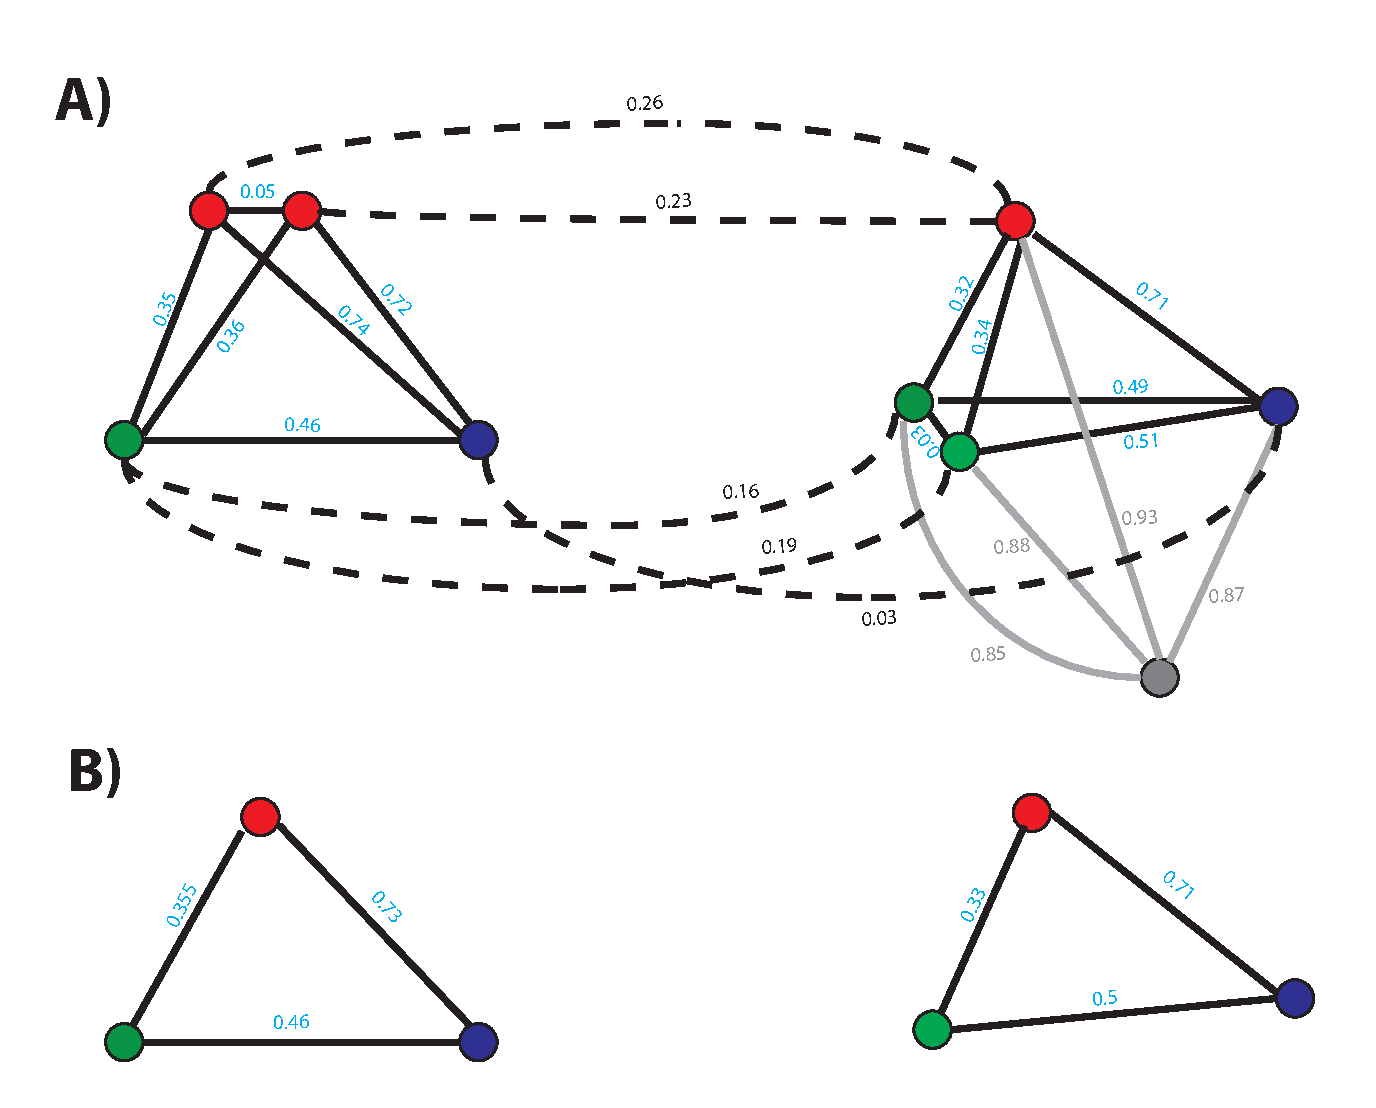
\includegraphics[scale=0.55]{graph_matching}
\caption{(A) An example dataset with a candidate matching. Circles represent clusters and node colors represent the matching. Dotted edges are used in the calcualtion of factor $A$. Grey edges from the unmatched grey cluster are used to calculate $C$. (B) An example collapsed graph from $A$. Differences between edges that connect the same colors are used to calculate $B$}
\end{figure}
Using the values in the figure above we would have:
$$
A = (0.26^2+0.23^2)/2 +(0.16^2+0.19^2)/2 + 0.03^2 = 0.092
$$

$$
B = (0.355 - 0.33)^2 + (0.73 - 0.71)^2 + (0.46 - 0.5)^2 = 0.002625
$$

$$
C = (0.85^2 +0.88^2 + 0.93^2 + 0.87^2)/4 = 0.779
$$

For $\sigma_1 = \sigma_2 = \sigma_3 = 1/3$, we have:
$$
Q = (A+B+C)/3 = 0.29121
$$

\section{Finding the optimal valid matching}
We propose the following greedy algorithm to find the optimal valid matching: 
We start out by calculating a maximum bipartite matching. In cases where there are no strong batch effects largely differentiating both datasets, bipartite matching is already a good candidate for the optimal matching. \\
\\
Starting from the initial matching, we successively swap colors of clusters to both existing and new colors - provided that the swapping preserves the valid matching property -. We then recalculate $Q$ and keep the color assignment that decreases $Q$ the most. This is a discrete analogy to the gradient descent method, where we iteratively shift our candidate minimum to the direction that minimizes the gradient of a given function. Much like the gradient descent, however, the algorithm is not guaranteed to converge to the global minimum. \emph{(However I'm crossing my fingers that the results in practical data will be satisfactory)}. Another possible option for the algorithm is to set multiple random starts as a matching and choose the one with best convergence of $Q$. \\
\\
We note, however, that this problem as it is phrased is computationally harder than the graph isomorphism problem, since, if we set $\sigma_1 = \sigma_3 = 0$ and $\sigma_2 = 1$ and the distance metric as a user-given one-zero adjacency matrix that defines the discrete edges between clusters, then comparing two equal datasets would be equivalent to finding the isomorphism  of two equal graphs, which is known to be NP-Complete. 
\\
\begin{algorithmic}
\Function{BipartiteMatching} {$X_1$, $X_2$, $||\cdot ||$}
	\State Find a maximum bipartite matching of the two datasets using edge weights as $1 - d$, where $d$ is the input distance matrix.
	\State Assign endpoints of all edges with the same color.
	\State Assign unique colors to nodes not connected by any edge.
	\State \Return $(c_1, c_2)$
\EndFunction
\\
\Function {OptimalValidMatching}{$X_1$, $X_2$, $||\cdot ||$}
	\State $(c_1,c_2) \gets$ \Call{BipartiteMatching}{$X_1$,$X_2$, $||\cdot ||$}
	\State $(S_1, S_2) \gets (Im(c_1), Im(c_2))$
	\State PossibleImprovemen $\gets$ true
	\While {PossibleImprovement == true}
		\State PossibleImprovement $\gets$ false
		\For {every cluster $x$ in $X_1 \cup X_2$}
			\For {every color $k$ in $S_1 \cup S_2$}
				\If {color of $x$ is not $k$}
					\State set color of $x$ as $k$
					\If {matching is still valid and $Q$ decreases}
						\State PossibleImprovement $\gets$ true
					\Else
						\State Set color of $x$ back to its original value
					\EndIf
				\EndIf
			\EndFor
			\If {assigning a new unused color to $x$ decreases $Q$}
				\State Set a new unused color to $x$
			\EndIf
		\EndFor
	\EndWhile
	\State \Return {$(c_1, c_2)$}
\EndFunction
\end{algorithmic}

\section{Distance Metrics}
%\subsection{Normalized Euclidean Distance}
%\subsection{Affinity Distance}
%\subsection{Pearson Correlation}

\section{Clustering Methods Used in Single Cell Analysis}
%\subsection{SNN-Modularity}
%\subsection{DBSCAN}
%\subsection{Gaussian Mixture Models}
%\subsection{Spectral Clustering}
%\subsection{K-Means}
%\subsection{Hierarchical Clustering}


\section{Previous Cluster Comparison Methods}

\subsection{CCLUMP}
% Jakobsson and Rosenberg

\subsection{MCES}
% Maximum common edge subgraph

\section{Data}
\begin{tabular}{ | c | c | c | c | c | p{6cm} | }
\hline
\textbf{Paper} & \textbf{Organism} & \textbf{Clustering} & \textbf{\# Clusters}& \textbf{\# Cells }& \textbf{\# Cells} \textbf{Details}\\
\hline
Yan & 
hg19 & 
Biological & 
7 & 
129 & 
Oocyte, Zygote, 2-cell, 4-cell, 8-cell, Morula, Blastocyst\\
\hline
Biase & 
mm10 & 
Biological & 
3 & 
56 & 
hESC, 2-cell, 4-cell\\
\hline
Goolam & 
mm10 & 
Biological & 
5 & 
40 & 
2-cell, 4-cell, 8-cell, Morula, Blastocyst\\
\hline
Deng & 
mm10 & 
Biological & 
10 &  
317& 
Oocyte, Zygote, 2-Cell(E,M,L), 4-cell, 8-cell,16-cell, Blastocyst(E,M,L)\\
\hline
Kolodziejczyk & 
hg19 & 
Biological & 
7 &
704   
& 
Oocyte, Zygote, 2-cell, 4-cell, 8-cell, Morula, Blastocyst\\
\hline
Pollen & 
hg19 & 
Biological & 
11 &  
301 & 
Brain Stuff\\
\hline
\hline
Macosko & 
hg19 & 
DBSCAN &  
&  
& Retina cells\\
\hline
Klein & 
mm10 & 
Marker Genes & 
4 & 
2,717 & 
Mouse ESC 1, 2, 4 and 7 days post LIF withdrawal \\
\hline
Shekhar & 
hg19 & 
SNN-Cliq &  
&  
& Retina cells\\
\hline
Zeisel & 
mm10 & 
BackSPIN &  
9 & 
3,005 & 
Brain cells\\
\hline

\end{tabular}

\end{document}